\documentclass[11pt]{article}

\usepackage{maiacustom}

\begin{document}

\psettitle{Banco de questões de astronomia}

Estas questões foram produzidas/selecionadas cuidadosamente com o objetivo de preparar os estudantes para o processo seletivo de astronomia no Brasil. Algumas questões não são de autoria própria e estão devidamente sinalizadas por () antes do enunciado. O template do banco de questões é o mesmo do Professor \text{Kevin Zhou}. Seu trabalho é valioso, e diversas ideias desta lista podem ser encontradas em seus Handouts.

% \begin{psidea}{Título da Ideia}{}
% Ideia
% \end{psidea}

% \begin{psexample}{Título do Exemplo}{}
% Exemplo
% \end{psexample}

% \begin{pssolution*}{}{}
% Solução
% \end{pssolution*}

% \begin{psremark*}{Título da Observação}{}
% Observação
% \end{psremark*} 
\section{Astronomia de Posição}

\pts{5} %problema da semana 114
\begin{pproblem} Após se perderem em uma navegação, você e o professor Klafke naufragam em uma ilha e encontram o seguinte relógio de Sol:
    \begin{figure}[H]
        \centering
        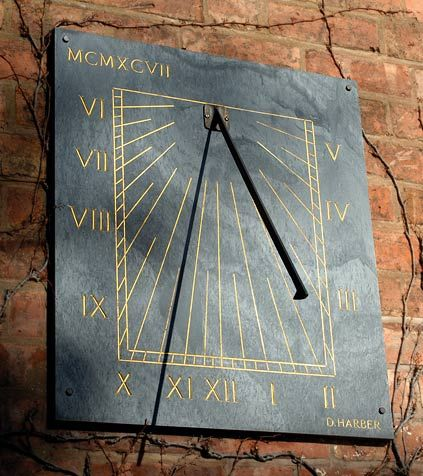
\includegraphics[width=0.5\linewidth]{imagens/q6.jpg}
        \caption{Relógio de Sol}
    \end{figure}
    Agora é missão de vocês descobrirem propriedades do relógio de Sol.
    \begin{enumerate}[label=\textbf{\alph*)}]
        \item Em qual hemisfério vocês se encontraram? Como você chegou a tal conclusão?
        \item Após várias semanas na ilha, vocês notam que a sombra do relógio parece seguir uma linha reta, sendo \(\phi\) a latitude que vocês se encontraram, determine a declinação do Sol nesse dia e explique o porquê disso só acontecer em \(2\) dias do ano.
        \item Prove que, quando o Sol possui a declinação encontrada anteriormente, a sombra segue uma linha reta. Isso pode ser feito seguindo os seguintes passos:
        \begin{enumerate}[label=\roman*)]
            \item Determine a orientação da linha e explique por que ela deve estar nessa orientação;
            \item Determine o comprimento da sombra para uma dada posição do Sol em coordenadas alt-azimute;
            \item Derive uma relação entre altitude e azimute, dado que a ponta da sombra está sobre a linha;
            \item Determine uma quantidade constante e mostre que ela é constante para todas as posições do Sol naquele dia.
        \end{enumerate}
    \end{enumerate}
\end{pproblem}

    \pts{5}
\begin{pproblem} (Adaptado T1 - 2024)
    A equação do tempo é a diferença entre a ascensão reta do Sol médio e a ascensão reta do Sol verdadeiro. Sabendo disso, vamos calcular algumas de suas propriedades.
    \begin{alternativas}
        \item Determine uma expressão para a equação do tempo, desconsiderando a excentricidade da Terra, i.e.: O Sol possuindo velocidade constante ao longo da eclíptica. Deixe sua resposta em função do tempo desde o equinócio de março \(T_M\), do período da Terra \(T\) e da obliquidade da eclíptica \(\epsilon\).
        \item Agora, considerando a excentricidade da Terra, a equação do tempo tem forma:
        \[E.T. = -2e \cdot \sin(k_1 \cdot M) + \tan^2 \left( \frac{\epsilon}{2} \right) \cdot \sin\left( k_2 \cdot (M + \lambda_P) \right)\]
        Onde \(M\) é a anomalia média, \(\lambda_P\) a longitude eclíptica do periastro e \(e\) a excentricidade da Terra. Determine as constantes \(k_1\) e \(k_2\). Pense nas situações de simetria envolvendo cada uma das parcelas da equação.
        \\
        Agora o objetivo da questão é descobrir a declinação do Sol no ponto de nó do analema. Veja a figura a seguir:
        \begin{figure}[H]
            \centering
            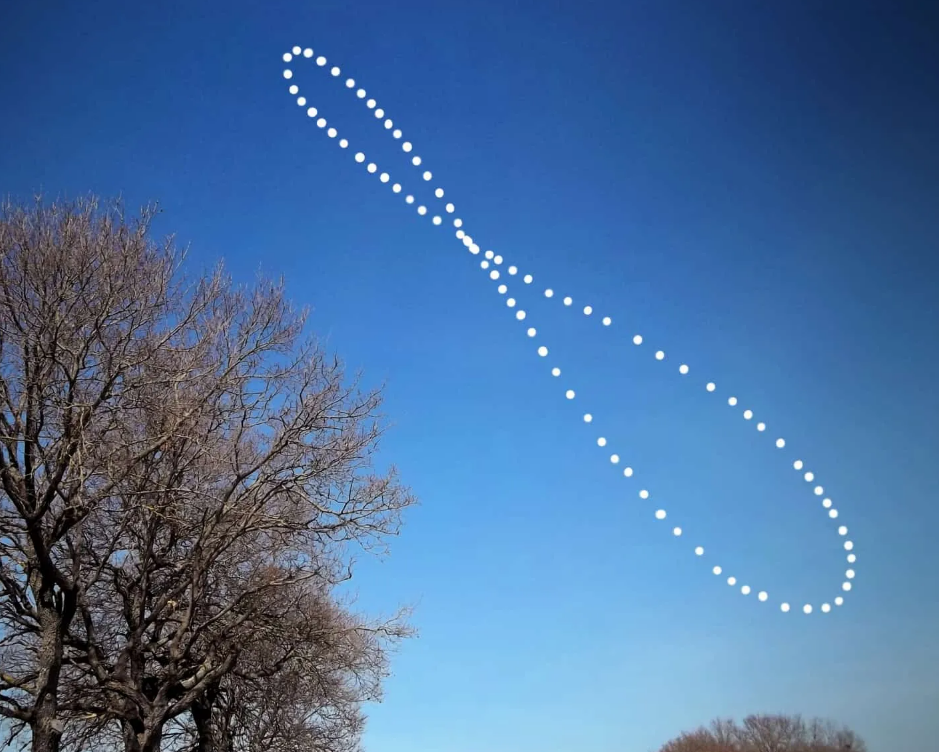
\includegraphics[width=0.7\textwidth]{imagens/q16.png}
            \caption{Representação analema}
        \end{figure}
        O ponto de nó é o ponto em que a trajetória se cruza.
        \item Para pequenos valores da declinação do Sol, obtenha uma fórmula para essa em função de \(M\), \(\lambda_P\) e \(\epsilon\). Considere também que a excentricidade e a inclinação da órbita sejam suficientemente pequenas.
        \item Encontre as duas anomalias médias que tenham a mesma declinação e mesma \(E.T.\).
        \item Encontre o valor da declinação solar no ponto de nó.
    \end{alternativas}
    \end{pproblem}

    
    \pts{5}
    \begin{pproblem}
        Porílio, após um longo dia de aulas no ITA, no solstício de verão (\(\phi = 23^\circ 11' S, \ \lambda = 45^\circ 53' O\)) deseja ver o por do Sol. No dia em questão, o valor da equação do tempo é \(E.T. = -3\) minutos. Porílio não quer perder o Sol de jeito nenhum e começa a correr para que o (centro do) Sol continue no horizonte.
    
        \begin{alternativas}
            \item São José dos Campos, segue o horário de Brasília (UTC-3h), em qual horário, no Tempo Civil, Porílio deve começar sua corrida?
            \item Se Porílio corre em direção a um dos polos geográficos, qual deve ser a sua velocidade inicial?
            \item Se Porílio decide subir uma montanha de inclinação \(i = 30^\circ\), a uma velocidade constante de \(v = 1\) m/s, qual o maior tempo com que Porílio consegue deixar o Sol acima do horizonte?
            \textbf{Dica: } Utilizar aproximações para pequenos ângulos, talvez seja útil.
        \end{alternativas}
\end{pproblem}

\pts{3}
\begin{pproblem}
    Mauí, um renomado astrônomo, deseja passar suas férias de fim de ano em Sergipe \((10^\circ \ 54'\ 33'' S, \ 37^\circ 4'29'' O\)) e deseja saber o horário de nascimento de uma de suas estrelas favoritas, All Kaf al Dij Ma \Romannum{3} \((\delta = +10^\circ \ 56'\ 58'', \ \alpha = 2h \ 58m \ 43s\)), e precisa de sua ajuda para calcular o horário de nascimento dela nas seguintes situações:
    
    \begin{alternativas}
        \item Calcule o horário de nascimento de All Kaf al Dij Ma \Romannum{3} no solstício de dezembro.
        \item Quanto tempo a estrela passará acima do horizonte?
        \item Estime o período de tempo em que a estrela é visível.
    \end{alternativas}

    \end{pproblem}

    \pts{4}
\begin{pproblem}(Lucas Cavalcante - \href{https://noic.com.br/olimpiadas/astronomia/problemas-da-semana/astronomia-semana-111/}{Semana 111})
    Considerando um sistema de coordenadas horizontal em que o azimute \(0\) corresponde ao ponto cardeal norte, um asteroide foi observado nas alturas \(h_1\) e \(h_2\) e azimutes \(A_1\) e \(A_2\), enquanto outro asteroide foi observado nas coordenadas \(h_3\), \(h_4\), \(A_3\) e \(A_4\). Encontre as coordenadas dos pontos de encontro entre os asteroides.
    
    \begin{psidea}{Notação de Einstein}{}
    Durante a resolução dessa questão, utilizarei a Notação de Einstein. Ela é uma ferramenta física para facilitar as contas vetoriais. Explicando, na notação comum, um vetor é representado por
    \[\mathbf{a} = (a_1 \hat{\mathbf{e}}_1, \ a_2 \hat{\mathbf{e}}_2, \ a_3 \hat{\mathbf{e}}_3)\]
    Na notação de Einstein, isso é substituído por:
    \[\mathbf{a} = a_i \hat{\mathbf{e}}_i\]
    Onde os índices repetidos indicam a soma (\(a_i \hat{\mathbf{e}}_i = a_1 \hat{\mathbf{e}}_1 + a_2 \hat{\mathbf{e}}_2 + a_3 \hat{\mathbf{e}}_3 + ...\))
    
    O produto escalar entre dois vetores, na notação de Einstein, é definido por:
    \[\mathbf{a}\cdot \mathbf{b} = a_i b_j \delta_{ij}\]
    Onde \(\delta_{ij}\) é a função \textit{Delta de Kronecker} e é definida por:
    \[\delta_{ij} = \left \{ \begin{matrix} 0, & \mbox{se } i \ne j \\ 
                                            1, & \mbox{se } i = j\end{matrix} \right.\]
    
    Assim, \(\mathbf{a}\cdot \mathbf{b} = a_i b_i \equiv a_1 b_1 + a_2 b_2 + a_3 b_3\)

    Já para o produto vetorial, temos:
        \[
        \mathbf{a} \times \mathbf{b} = a_i b_j \Epsilon_{ijk} \hat{\mathbf{e}}_k
        \]
        Aqui, \(\Epsilon_{ijk}\) é denominado \textit{tensor de Levi-Civita}, ou símbolo de Levi-Civita, e é definido como:
    
        \[
        \Epsilon_{ijk} = 
        \begin{cases} 
        +1 & \text{se } (i, j, k) \text{ é uma permutação par de } (1, 2, 3), \\
        -1 & \text{se } (i, j, k) \text{ é uma permutação ímpar de } (1, 2, 3), \\
        0 & \text{se dois ou mais índices são iguais}.
        \end{cases}
        \]

        Por exemplo, \(\Epsilon_{123} = \Epsilon_{312} = \Epsilon_{231} = 1\) e \(\Epsilon_{132} = \Epsilon_{213} = \Epsilon_{321} = -1\).
        Explicitamente 
        \[\mathbf{a} \times \mathbf{b} = (a_2 b_3 - a_3 b_2) \hat{\mathbf{e}}_1 + (a_3 b_1 - a_1 b_3) \hat{\mathbf{e}}_2 + (a_1 b_2 - a_2 b_1) \hat{\mathbf{e}}_3\]
    \end{psidea}
\end{pproblem}


\pts{5}
\begin{pproblem} (Lista \(1\) - Vinhedo 2024) Considere um relógio de Sol composto por um mostrador vertical
    e um gnômon, conforme mostrado na figura.
    \begin{figure}[H]
        \centering
        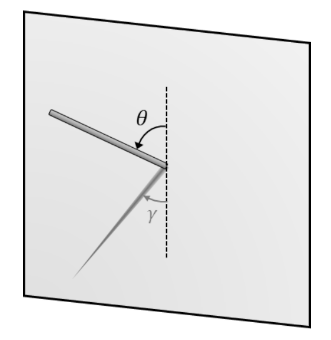
\includegraphics{imagens/q20.png}
        \caption{Esquema relógio de Sol.}
    \end{figure}
    \begin{alternativas}
        \item Suponha um relógio de Sol vertical cujo gnômon esteja corretamente apontado para o sul.
        Seja \(\phi\) a latitude do observador, \(H\) o ângulo horário do Sol e \(\delta\) a declinação solar. Determine
        a relação entre \(\theta\) e \(\gamma\) em função dessas variáveis.
        
        \item Com base no item anterior, qual deve ser o valor de \(\theta\) para que o relógio funcione durante o ano todo?

        \item Utilizando o valor correto para \(\theta\), determine a relação entre \(\gamma\) e \(H\), em função de \(\phi\) apenas.
    \end{alternativas}
\end{pproblem}


\pts{2} 
\begin{pproblem}
    Qual a menor altura que um gigante (que vive MUITOS), localizado no polo Sul, precisa ter para conseguir ver todas as estrelas do céu?
\end{pproblem}


\pts{3}
\begin{pproblem}
    Toleduardo deseja ver o pôr do Sol, mas acabou passando tempo demais na SorveterITA. Toleduardo é um homem \textit{Just in time} e deseja saber quanto tempo o pôr do Sol vai durar, para que ele possa se atrasar com calma. Sabendo que Toleduardo só vai para a SorveterITA nos dias 21 de março ou 22 de setembro, calcule qual é a duração do pôr do Sol na SorveterITA.
    \\
    \textbf{Dados: } Latitude da SorveterITA \(\phi = 23^\circ \ 10' \ 45''S, \ \ \lambda = 45^\circ 53' 14''O\).
\end{pproblem}


\pts{3}
\begin{pproblem} (Lista 2 - Vinhedo 2021)
    Em fevereiro de 2015, a Lua iniciou um ciclo de ocultações mensais de Aldebaran ($\alpha$ Tau). Ou seja, todo mês a Lua passava na frente de Aldebaran para um observador na Terra. Vale ressaltar que essas ocultações não ocorriam necessariamente para observadores na mesma posição todo mês. 

    Calcule a data (mês e ano) do fim desse ciclo de ocultações mensais. Considere que a órbita da Lua é circular.

    \subsection*{Dados:}

    \begin{itemize}
        \item Latitude eclíptica de Aldebaran = $5,47^\circ$
        \item Período de precessão nodal da Lua = 18,6 anos
    \end{itemize}
\end{pproblem}


\pts{4}
\begin{pproblem} (Lista 2 - Vinhedo 2021)
    Miguel vive em uma ilha isolada no Oceano Pacífico Sul, em uma longitude
    $\lambda = 176^{\circ}09^{\prime}137,7^{\prime\prime}\text{W}$. Ao longo do ano, o local onde o Sol nasce, visto por Miguel, varia $\Delta A = 67^{\circ}03^{\prime}81^{\prime\prime}$ no horizonte. Para os dois primeiros itens, desconsidere a refração atmosférica. Com essas informações, descubra:

    \begin{alternativas}
        \item A latitude $\phi$ e o nome da ilha. (Consulte o Google Earth ou software similar)
        \item O intervalo de horários em que o Sol nasce na ilha, dado o fuso horário peculiar $UT + 12\frac{3}{4}$.
        \item Considerando a refração atmosférica, o tamanho do intervalo do item anterior iria diminuir, aumentar ou se manter constante?
    \end{alternativas}

\end{pproblem}


\pts{3}
\begin{pproblem}(Lista 2 - Vinhedo 2022) 
    Bruno decidiu alugar uma casa para passar as férias em Cuiabá ($15,3^{\circ} \text{S}$, $56,1^{\circ} \text{O}$). Como um bom astrônomo, Bruno passava suas noites sentado em uma cadeira observando as estrelas por uma porta gigante voltada para o ponto cardeal sul.

    A porta tinha 4,00 metros de altura e 1,50 metros de largura. Bruno tinha o costume de sentar a
    1,00 metro da porta perfeitamente alinhado com o seu centro na horizontal. Ou seja, o segmento
    de reta entre os olhos de Bruno e o ponto que está exatamente no meio da porta na horizontal e
    na altura dos olhos forma um ângulo de $90^{\circ}$ com o plano da porta. Os olhos de Bruno ficam a
    1,20 metros do chão quando ele está sentado na cadeira.
    
    Para facilitar as suas observações, Bruno criou um sistema de coordenadas baseado na posição da
    porta, de onde ele via as estrelas a partir do local onde estava sentado, utilizando metros como
    a unidade de referência. A origem do sistema está localizada no canto inferior esquerdo. As coordenadas
    em $x$ aumentam para a direita e as coordenadas em $y$ aumentam para cima. Dessa forma, uma
    estrela vista a 1 metro do lado esquerdo da porta e 2 metros acima do chão seria representada
    pelas coordenadas $(1, 2)$.
    
    Bruno estava bastante interessado em Shaula ($\lambda \ \text{Sco}, \delta = 37,1^{\circ} \text{S}$). Determine as coordenadas de
    Shaula no instante em que a estrela se tornava visível para Bruno quando observada através da porta. Assuma que Shaula estava abaixo do horizonte quando Bruno começava a observar o céu.
\end{pproblem}


\end{document}